\chapter{Конструкторская часть}

В данном разделе представлена разработка функциональной модели (IDEF0) программного обеспечения, а также разработка алгоритмов выбора символов для представления формы, выбора символов для представления яркости, закраски методом Гуро, алгоритма удаления невидимых рёбер и поверхностей, использующего Z-буфер и используемых типов и структур данных.

\section{Разработка функциональной модели (IDEF0) ПО}

На рисунках \ref{fig:idef0-1}-\ref{fig:idef0-3} представлена декомпозиция разрабатываемого ПО в нотации IDEF0.

\begin{figure}[H]
    \centering
    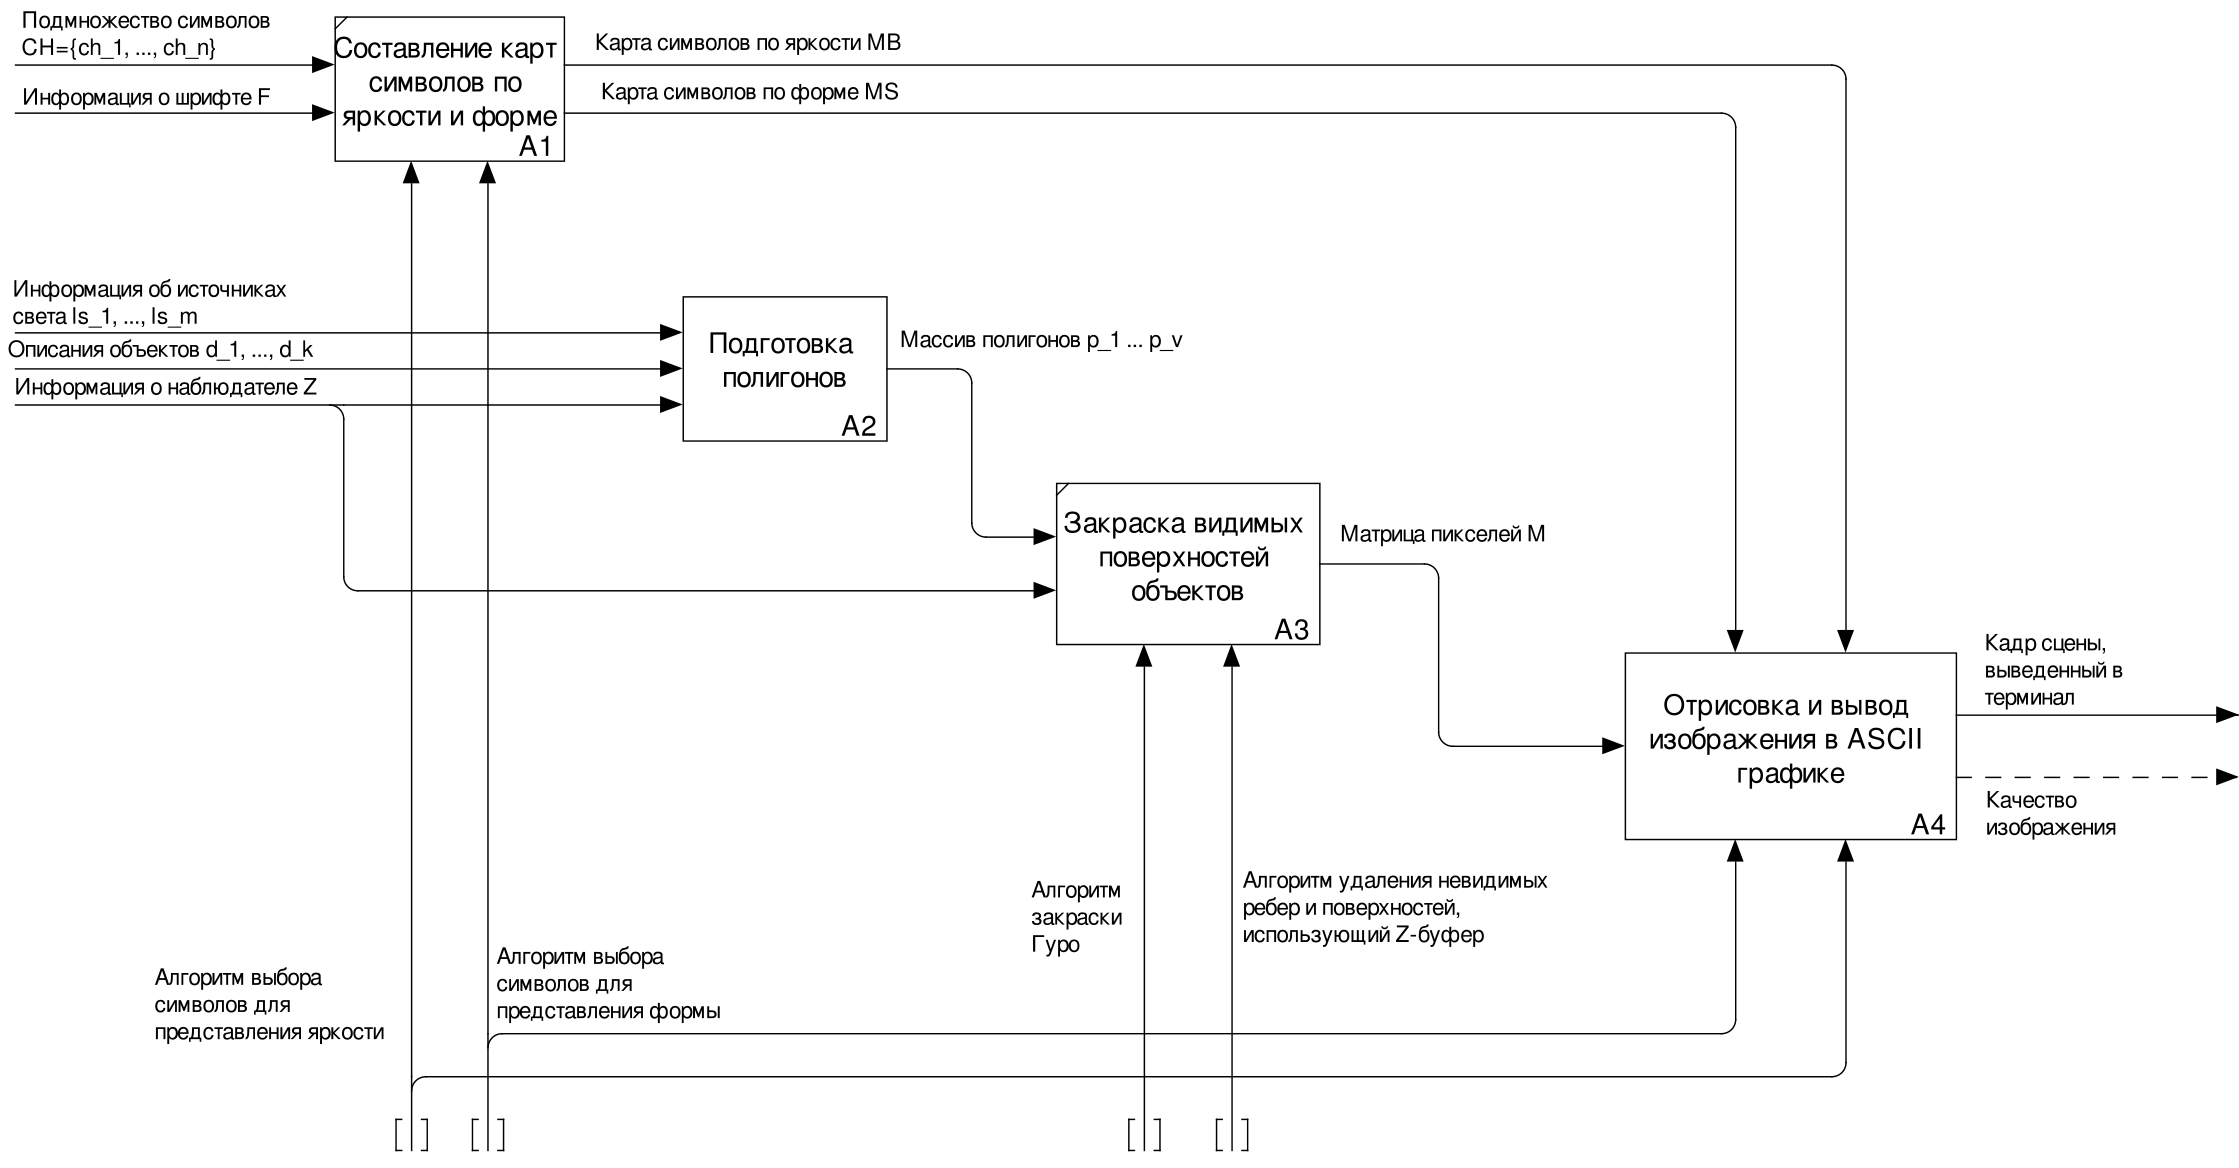
\includegraphics[scale=0.2]{images/02_A0.png}
    \caption{3D визуализатор каркасных объектов и эллипсоидов, использующий ASCII графику}
    \label{fig:idef0-1}
\end{figure}

\begin{figure}[H]
    \centering
    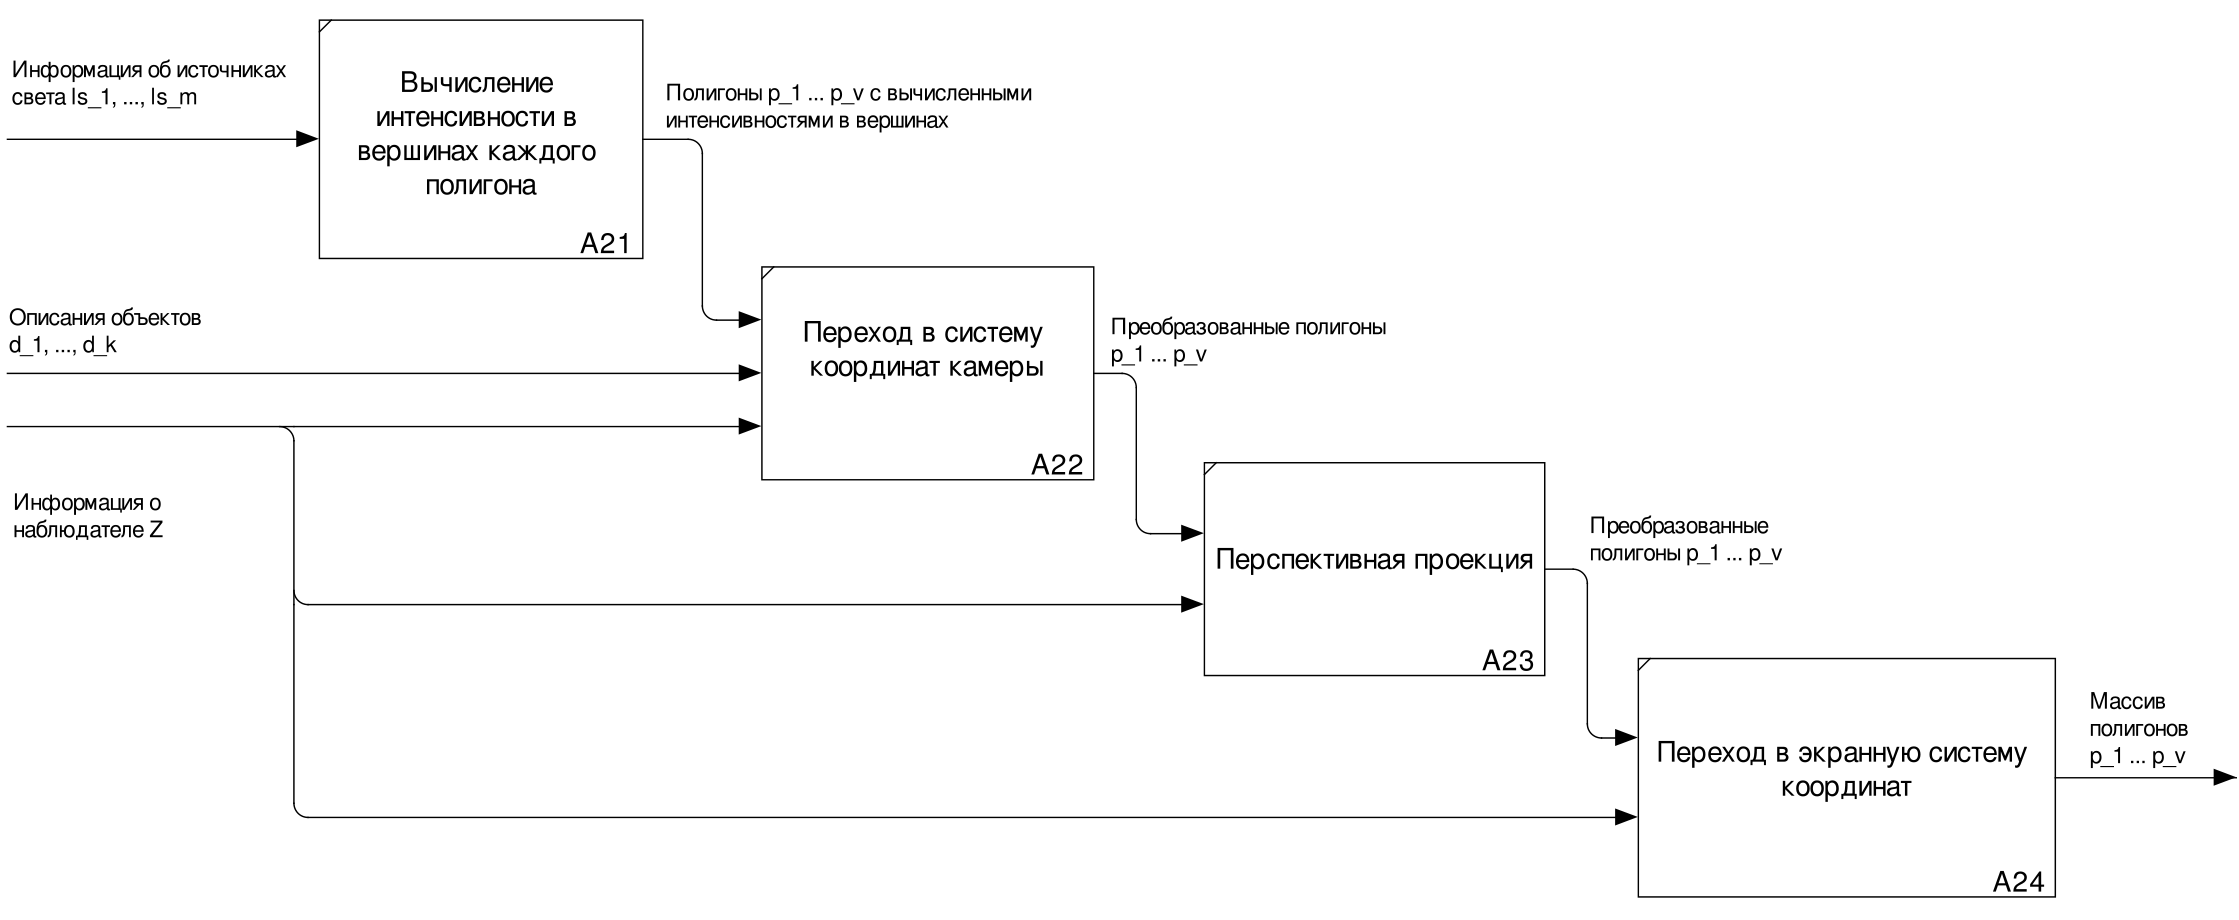
\includegraphics[scale=0.2]{images/03_A2.png}
    \caption{Подготовка полигонов}
    \label{fig:idef0-2}
\end{figure}

\begin{figure}[H]
    \centering
    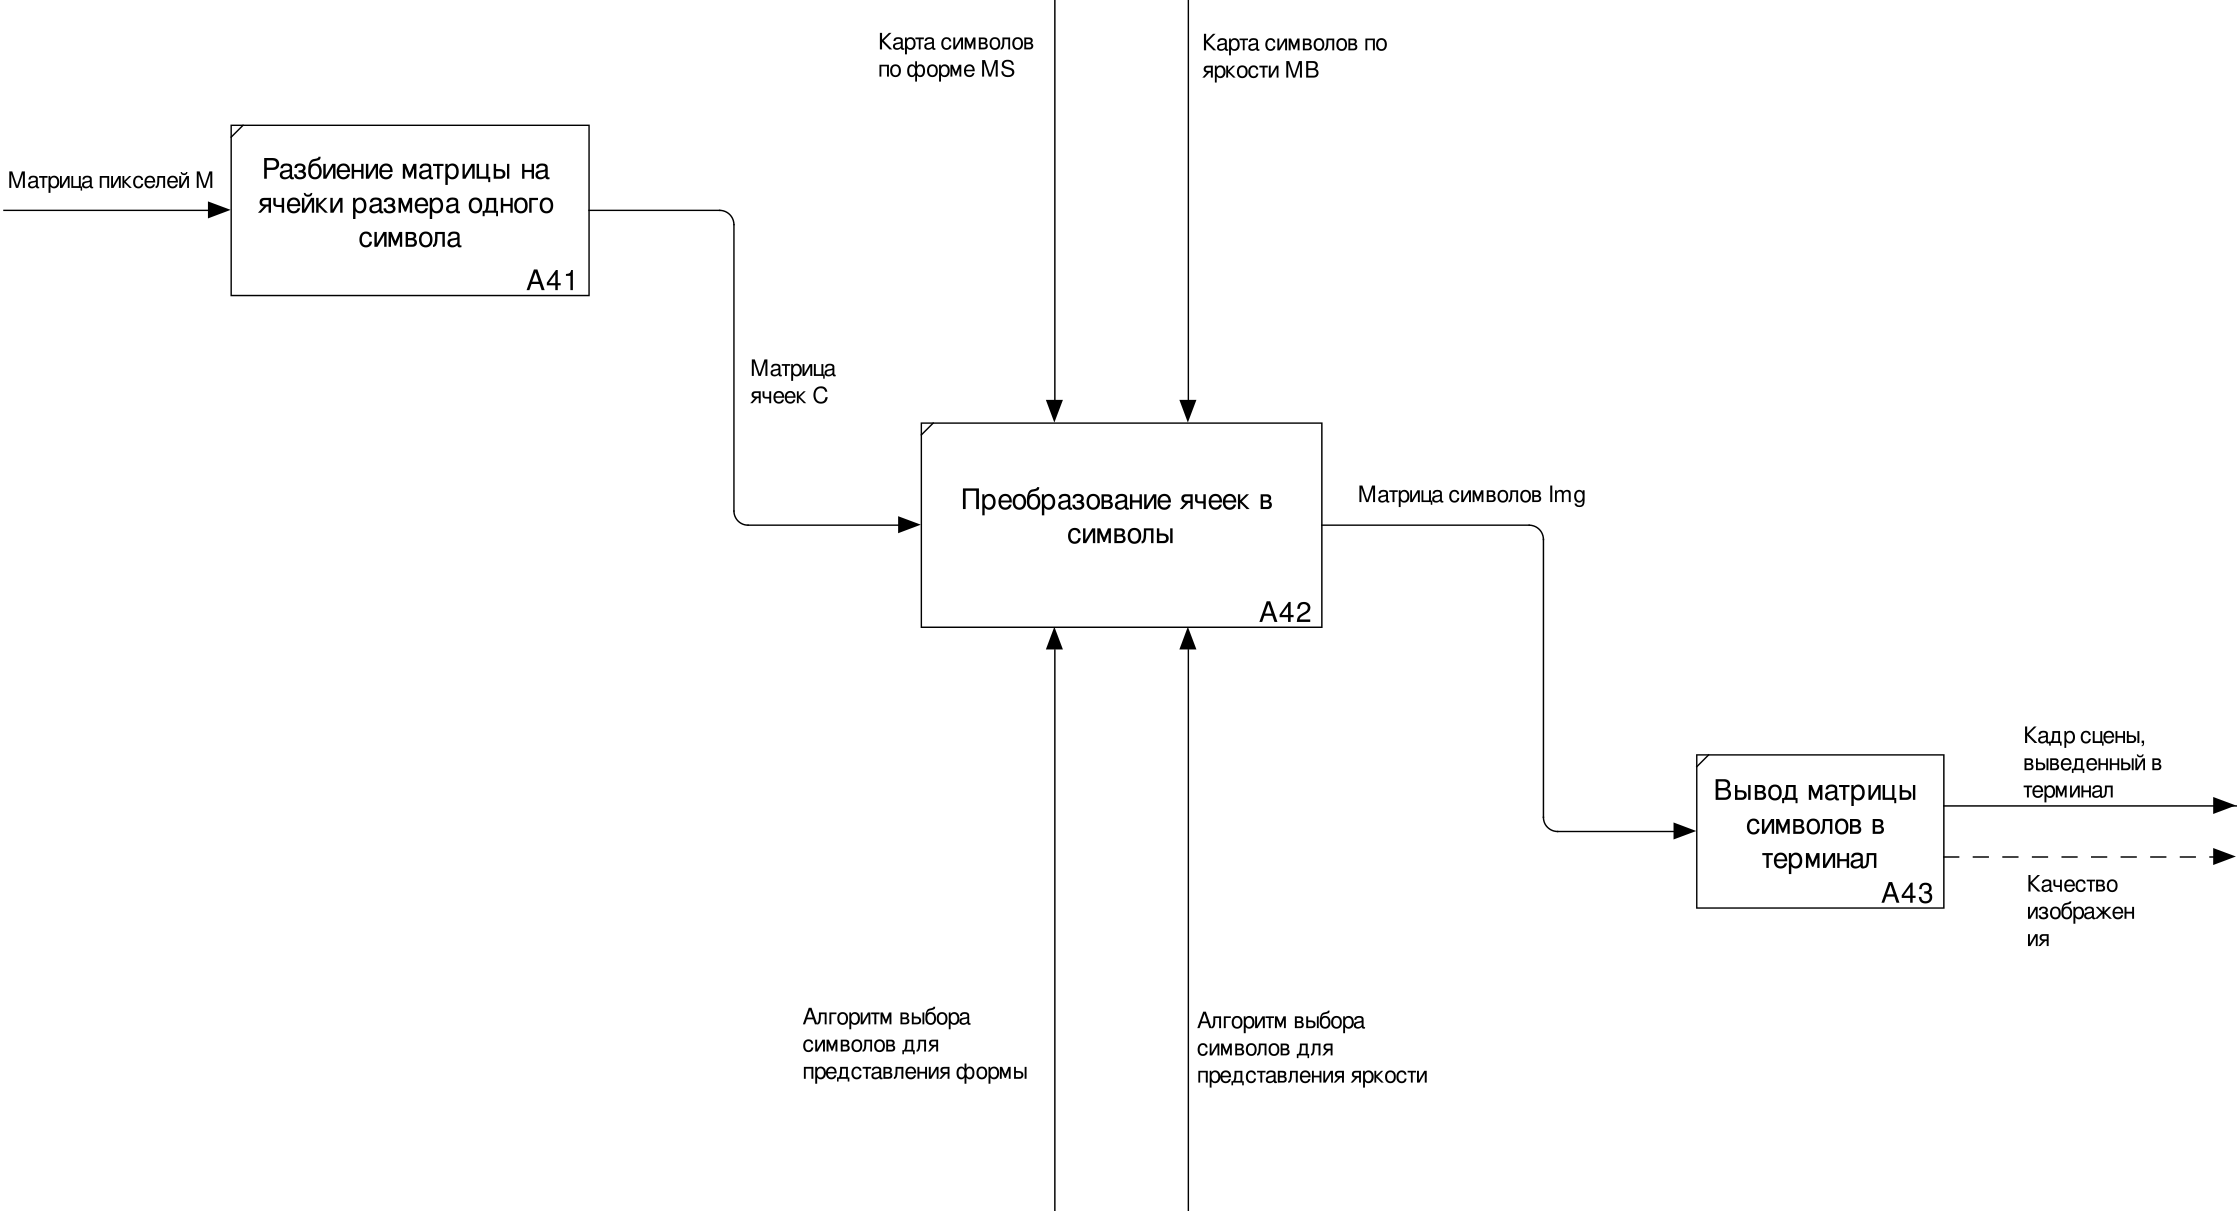
\includegraphics[scale=0.2]{images/04_A4.png}
    \caption{Отрисовка и вывод изображения в ASCII графике}
    \label{fig:idef0-3}
\end{figure}

\section{Получение информации о шрифте}

Для алгоритмов выбора символов для представления формы и яркости необходима информация о используемом в терминале шрифте в виде матриц пикселей каждого символа ASCII. Для этого необходим алгоритм обработки файлов шрифта. В файлах шрифта хранится векторное представление символов, которое необходимо преобразовать в растровое.~\cite{ttf}

\textbf{Алгоритм получения информации о шрифте:}

\textbf{Входные данные:}
\begin{itemize}
    \item описание шрифта $F$:
    \begin{itemize}
        \item векторные представления символов ASCII $V$=$v_1, ... v_m$;
        \item размер символа в терминале $x$ на $y$;
    \end{itemize}
    \item множество символов $CH=\{ch_1, ..., ch_n\}$.
\end{itemize}

\textbf{Возвращаемые данные:} карта $MF$ матриц пикселей для каждого символа множества $CH$

\textbf{Алгоритм:}

\begin{enumerate}
    \item для каждого символа $ch_i$ из множества $CH$:
    \begin{itemize}
        \item получение векторного представления $v$ из $V$ для символа $ch_i$;
        \item создание пустой матрицы размера $x$ на $y$;
        \item отрисовка символа в рамках матрицы по $v$;
        \item запись полученной матрицы в карту $MF$ в соответствие символу $ch_i$.
    \end{itemize}
    \item возврат карты $MF$.
\end{enumerate}

\section{Разработка алгоритма выбора символов для представления формы}

\textbf{Построение описательного вектора}

\textbf{Входные данные:}
\begin{itemize}
    \item матрица пикселей $M$;
    \item параметры аппроксимации $ctx$: 
    \begin{itemize}
        \item количество разбиений ячейки по вертикали $vertParts$;
        \item количество разбиений ячейки по горизонтали $horParts$;
        \item сектора полярной диаграммы $phiParts$;
        \item количество разбиений сектора $rParts$;
        \item максимальная длина сектора $rMax$.
    \end{itemize}
\end{itemize}

\textbf{Возвращаемые данные:} описательный вектор $v$

\textbf{Алгоритм:}

\begin{enumerate}
    \item $v$ = пустой описательный вектор;
    \item $n$ = ширина матрицы $M$;
    \item $m$ = высота матрицы $M$;
    \item $nStep$ = $n$ / $horParts$;
    \item $mStep$ = $m$ / $vertParts$;
    \item $rStep$ = $rMax$ / $rParts$;
    \item $phiStep$ = 2 * $\pi$ / $phiParts$;
    \item для каждого участка матрицы (по шагам $nStep$ и $mStep$);
    \begin{itemize}
        \item $currHyst$ = матрица размера $rParts~\times~phiParts$;
        \item для каждого сектора полярной диаграммы (i по $phiStep$ и j по $rStep$):
        \begin{itemize}
            \item если хотя бы один пиксель из $MF$ находится в секторе:
            \item $currHyst[i][j]$ = 1;
            \item иначе;
            \item $currHyst[i][j]$ = 0.
        \end{itemize}
        \item добавление $currHyst$ в $resVector$.
    \end{itemize}
    \item возврат $v$.
\end{enumerate}

\textbf{Построение карты $MS$ символов по форме:}

\textbf{Входные данные:}
\begin{itemize}
    \item карта $MF$ матриц пикселей для каждого символа множества $CH$;
    \item параметры аппроксимации $ctx$: 
    \begin{itemize}
        \item количество разбиений ячейки по вертикали $vertParts$;
        \item количество разбиений ячейки по горизонтали $horParts$;
        \item сектора полярной диаграммы $phiParts$;
        \item количество разбиений сектора $rParts$;
        \item максимальная длина сектора $rMax$.
    \end{itemize}
\end{itemize}

\textbf{Возвращаемые данные:} карта $MS$ символов по форме

\textbf{Алгоритм:}

\begin{enumerate}
    \item для каждого символа $ch_i$ карты $MF$:
    \begin{itemize}
        \item построение описательного вектора $v$ с параметрами $ctx$;
        \item запись полученного вектора $v$ в карту $MS$ в соответствие символу $ch_i$.
    \end{itemize}
    \item возврат $MS$.
\end{enumerate}

\textbf{Подбор символа в соответствие ячейке:}

\textbf{Входные данные:}
\begin{itemize}
    \item матрица пикселей ячейки $C_i$;
    \item карта $MS$ символов по форме;
    \item параметры аппроксимации $ctx$: 
    \begin{itemize}
        \item количество разбиений ячейки по вертикали $vertParts$;
        \item количество разбиений ячейки по горизонтали $horParts$;
        \item сектора полярной диаграммы $phiParts$;
        \item количество разбиений сектора $rParts$;
        \item максимальная длина сектора $rMax$.
    \end{itemize}
\end{itemize}

\textbf{Возвращаемые данные:} символ $cRes$

\textbf{Алгоритм:}

\begin{enumerate}
    \item построение описательного вектора $v$ для $C_i$ с параметрами $ctx$;
    \item $cRes$ - символ;
    \item $mindelt$ = $\infty$;
    \item для каждого описательного вектора $cv_i$ символа $ch_i$ из карты $MS$:
    \begin{itemize}
        \item $d$ = 0;
        \item для каждой $i$-й гистограммы $v$:
        \begin{itemize}
            \item $d$ = $d$ + ||$v[i]$ - $cv_i[i]$||.
        \end{itemize}
        \item если $d$ < $mindelt$:
        \begin{itemize}
            \item $mindelt$ = $d$;
            \item $cRes$ = $ch_i$.
        \end{itemize}
    \end{itemize}
    \item возврат $cRes$.
\end{enumerate}

\section{Разработка алгоритма выбора символов для представления яркости}

\textbf{Построение карты $MB$ символов по яркости:}

\textbf{Входные данные:} карта $MF$ матриц пикселей для каждого символа множества $ChS$

\textbf{Возвращаемые данные:} карта $MB$ символов по яркости

\textbf{Алгоритм:}

\begin{enumerate}
    \item $maxCnt$ = 0
    \item для каждого символа $ch_i$ карты $MF$:
    \begin{itemize}
        \item $cnt$ = количество пикселей символа $ch_i$
        \item если $cnt$ > $maxCnt$
        \begin{itemize}
            \item $maxCnt$ = $cnt$
        \end{itemize}
    \end{itemize}
    \item для каждого символа $ch_i$ карты $MF$:
    \begin{itemize}
        \item $cnt$ = количество пикселей символа $ch_i$
        \item запись $cnt / maxCnt$ в карту $MB$ в соответствие символу $ch_i$
    \end{itemize}
    \item возврат $MB$.
\end{enumerate}

\textbf{Подбор символа в соответствие ячейке:}

\textbf{Входные данные:}
\begin{itemize}
    \item яркость $b$ ячейки $C$;
    \item карта $MB$ символов по яркости.
\end{itemize}

\textbf{Возвращаемые данные:} символ $cRes$

\textbf{Алгоритм:}

\begin{enumerate}
    \item $cRes$ - символ;
    \item $mindelt$ = $\infty$;
    \item для каждого значения яркости $cb_i$ символа $ch_i$ из карты $MB$:
    \begin{itemize}
        \item $d$ = $|cb_i - b|$;
        \item если $d$ < $mindelt$:
        \begin{itemize}
            \item $mindelt$ = $d$;
            \item $cRes$ = $ch_i$.
        \end{itemize}
    \end{itemize}
    \item возврат $cRes$.
\end{enumerate}

\section{Разработка алгоритма закраски методом Гуро}

\textbf{Входные данные:}
\begin{itemize}
    \item грань $f$ объекта, заданная вершинами $\{v_1, v_2, v_3\}$ и нормалями $\{\mathbf{n}_1, \mathbf{n}_2, \mathbf{n}_3\}$ в этих вершинах;;
    \item массив источников света $ls_1, ..., ls_m$, где каждый источник $ls_i$ задан позицией $\mathbf{p}_i$ и интенсивностью $I_i$.
\end{itemize}

\textbf{Возвращаемые данные:} закрашенный полигон $p$.

\textbf{Алгоритм:}

\begin{enumerate}
    \item инициализация итоговой интенсивности для каждой вершины: $I(v_i) \gets k_a$, где $i = 1, 2, 3$;
    \item для каждой вершины $v_i$ с нормалью $\mathbf{n}_i$:
    \begin{itemize}
        \item для каждого источника света $ls_j$:
        \begin{itemize}
            \item $\mathbf{l}_j = \frac{\mathbf{p}_j - v_i}{\|\mathbf{p}_j - v_i\|}$;
            \item если $\mathbf{n}_i \cdot \mathbf{l}_j \leq 0$, перейти к следующему источнику;
            \item $I_d = k_d \cdot I_j \cdot \max(0, \mathbf{n}_i \cdot \mathbf{l}_j)$;
            \item $\mathbf{r}_j = 2(\mathbf{n}_i \cdot \mathbf{l}_j)\mathbf{n}_i - \mathbf{l}_j$;
            \item $I_s = k_s \cdot I_j \cdot \max(0, (\mathbf{r}_j \cdot \mathbf{v}_{obs})^n)$;
            \item $I(v_i) \mathrel{+}= I_d + I_s$.
        \end{itemize}
    \end{itemize}
    \item для каждого пикселя внутри треугольника $f$:
    \begin{itemize}
        \item $(\alpha, \beta, \gamma) = \text{ComputeBarycentric}(x, y, v_1, v_2, v_3)$;
        \item $I(x, y) = \alpha \cdot I(v_1) + \beta \cdot I(v_2) + \gamma \cdot I(v_3)$;
        \item закрасить пиксель $(x, y)$ с интенсивностью $I(x, y)$.
    \end{itemize}
    \item возврат $p$.
\end{enumerate}

\section{Разработка алгоритма удаления невидимых ребер и поверхностей, использующего Z-буфер}

\textbf{Входные данные:}
\begin{itemize}
    \item массив полигонов $p_1, ..., p_v$;
    \item высота $h$ и ширина $w$ изображения.
\end{itemize}

\textbf{Возвращаемые данные:} матрица пикселей изображения $M$.

\textbf{Алгоритм:}

\begin{enumerate}
    \item создание буфера изображения $img$ - матрицы пикселей размера $h\times w$;
    \item создание Z-буфера $zBuf$ - матрицы вещественных чисел размера $h\times w$, заполненной максимальными возможными значениями $z$;
    \item для каждого пикселя $px_i$ каждого полигона $p_i$:
    \begin{itemize}
        \item если $(0 \leq x < w, \quad 0 \leq y < h)$ И $(zBuf[y][x] > z)$:
        \begin{itemize}
            \item $img[y][x] = \text{пиксель}$;
            \item $zBuf[y][x] = z$.
        \end{itemize}
    \end{itemize}
    \item возврат $img$.
\end{enumerate}

\section{Разработка типов и структур данных}

\begin{itemize}
    \item структура объекта содержит:
    \begin{itemize}
        \item массив граней модели $Faces$;
        \item центр модели $Center$ (три вещественных переменных).
    \end{itemize}
    \item структура грани содержит:
    \begin{itemize}
        \item массив координат вершин $Vertices$;
        \item массив нормалей к вершинам $Normals$.
    \end{itemize}
    \item структура пикселя содержит:
    \begin{itemize}
        \item яркость $brightness$, представленную вещественным числом от 0 до 1;
        \item флаг $isPolygon$, показывающий, является ли пиксель частью полигона;
        \item флаг $isLine$, показывающий, является ли пиксель частью ребра.
    \end{itemize}
    \item структура полигона содержит набор пикселей, сопоставленных координатам экрана;
    \item структура камеры содержит:
    \begin{itemize}
        \item координату на оси $Z$, задающую ее положение;
        \item угол обзора камеры $fov$;
        \item соотношение сторон камеры $aspect$;
        \item координату $zFar$ дальней плоскости обрезания;
        \item координату $zNear$ ближней плоскости обрезания.
    \end{itemize}
    \item структура источника света содержит:
    \begin{itemize}
        \item координаты положения источника света в пространстве $Position$ (три вещественных переменных);
        \item интенсивность излучения $Intensity$ (вещественная переменная).
    \end{itemize}
\end{itemize}

\section{Выводы из конструкторской части}

Было спроектировано программное обеспечение, разработаны алгоритмы выбора символов для представления формы, выбора символов для представления яркости, закраски методом Гуро, удаления невидимых рёбер и поверхностей с использованием Z-буфера и типы и структуры данных.

\clearpage
